\documentclass[a4paper,14pt]{article}
\usepackage[utf8]{inputenc}
\usepackage[russian]{babel} 
\usepackage{graphicx} 
\usepackage{amsmath}
\usepackage{amssymb}
\usepackage{siunitx}% Для погрешностей
\usepackage{float}
\usepackage[colorlinks=true, linkcolor=blue]{hyperref}
\usepackage{enumitem}
\usepackage{longtable}
\usepackage[left=2.5cm, right=1.5cm]{geometry}
%\documentclass[fleqn]{article}
% Подключаем пакет для управления колонтитулами
\usepackage{scrlayer-scrpage}
\pagestyle{plain}



\begin{document}

\begin{titlepage}
    \newpage
    \centering

    МИНИСТЕРСТВО ОБРАЗОВАНИЯ И НАУКИ РОССИЙСКОЙ ФЕДЕРАЦИИ\\
    \textbf{ФЕДЕРАЛЬНОЕ ГОСУДАРСТВЕННОЕ АВТОНОМНОЕ ОБРАЗОВАТЕЛЬНОЕ УЧРЕЖДЕНИЕ ВЫСШЕГО ОБРАЗОВАНИЯ \\
    «НОВОСИБИРСКИЙ НАЦИОНАЛЬНЫЙ
    ИССЛЕДОВАТЕЛЬСКИЙ ГОСУДАРСТВЕННЫЙ УНИВЕРСИТЕТ».}\\
    \vspace{0.5cm}
    \textbf{Физический факультет}



    \vspace{4cm}

    {\Large \textbf{Отчет о работе}} \\
    \vspace{0.5cm}
    {\large «ИЗМЕРЕНИЕ СТАЦИОНАРНЫХ СЛУЧАЙНЫХ ВЕЛИЧИН И СТАТИСТИЧЕСКАЯ ОБРАБОТКА
    РЕЗУЛЬТАТОВ ИЗМЕРЕНИЙ»}

    \vspace{3cm}

    \begin{flushright}
        Выполнил: студент группы №26311 \\
        Батанин Артём Александрович \\
        Работа выполнена в рамках курса\\
        «Обработка данных физического эксперимента»
        \vspace{1cm}

        «15» Ноября 2026г.

        \vspace{1cm}

        Оценка: \rule{3cm}{0.4pt} \\
        Преподаватель Васильев А.В. \\
        «\rule{0.5cm}{0.4pt}» \rule{3cm}{0.4pt} 2026г.
    \end{flushright}

    \vfill

    Новосибирск 2026

\end{titlepage}


\pagestyle{scrheadings}

%\clearpagemainheadfoot % Очищаем стандартные колонтитулы
\cfoot{\thepage}
% Настраиваем верхний правый угол (Right Head)
\rofoot{
\includegraphics[width=2.5cm]{Mir_insignia.png}}
% Вместо \rohead можно использовать:
% \lehead (левый верхний), \rofoot (правый нижний), \lefoot (левый нижний)


%\maketitle

%\newpage
\tableofcontents    
\newpage            

\section{Описание работы}
\subsection{Цель работы}
Цель работы – ознакомление с методами обработки и представления
результатов измерений случайных величин на примере исследования интенсивности излучения $\alpha$-частиц при радиоактивном распаде ядер.

\subsection{Оборудование}
Оборудование: источник $\alpha$-частиц (алюминиевая подложка с солями $ ^{239}Pu$), сцинтиллятор, фото-электронный умножитель, пересчетное устройство, компьютер.



\section{Теоретическое описание}
 $ ^{239}Pu$ распадается на $^4\alpha^{++}$ и $^{235}U$. Ядра плутония распадаются независимо друг от друга: распад одного ядра не может повлиять на другое т.к.
при распаде выделяется только альфа частица которая не может проникнуть свкозь электронную оболочку атома к ядру.

Для отдельно взятого ядра (вещества с периодом полураспада T) вероятность распасться за время t:

\begin{equation}
\begin{aligned}
P = 1 - 2^{-\frac{t}{T}}
 \label{eq:prob1}
 \end{aligned}
\end{equation}

Для образца из N атомов ожидаемое число распадов: $\bar{N}_{\text{расп}} = N(1 - 2^{-\frac{t}{T}})$.
В эксперименте проводилось измерение количества распадов за некоторый промежуток времени t.
Период полураспада $ ^{239}Pu$ около 24 тысяч лет - в рамках
данной работы работы рассматриваются промежутки времени значительно меньше. Оценим вклад изменения массы образца за время эксперимента на итоговый результат:

За 1 день распадется  $m_0\cdot (1 - e^{-\frac{1}{24000\cdot 360}}) \approx m_0\cdot 10^{-7}$. Влияением данного фактора можно пренебречь т.к. он на несколько порядков меньше
статистической неопределенности, рассмотренной ниже.

Посчитаем вероятность зарегестрировать n распадов за время t при помощи бинома Ньютона:

\begin{equation}
\begin{aligned}
P_n = C^n_N\cdot(1-2^{-\frac{t}{T}})^n\cdot (2^{-\frac{t}{T}})^{N-n}
 \label{eq:prob2}
 \end{aligned}
\end{equation}


Т.к. $N\rightarrow\infty$;  $P\rightarrow0$, приведенное выше биноминальное распределение будет стремиться к распределению Пуассона:

\begin{equation}
\begin{aligned}
P_n = \frac{\lambda^n}{n!}e^{-\lambda}
 \label{eq:puasson}
 \end{aligned}
\end{equation}



В экспериментах с большим временем экспозиции ($\delta t > 50$мс) среднее количество распадов ($\lambda$) больше 90,
вероятность каждого отдельного исхода уже становится значимой, в таком случае распределение количества распадов за экспозицию
стремится к нормальному распределению.
Также это следует из центральной предельной теоремы - сумма независимых случайных величин имеет расапределение близкое к нормальному.


\begin{figure}[H]
\centering
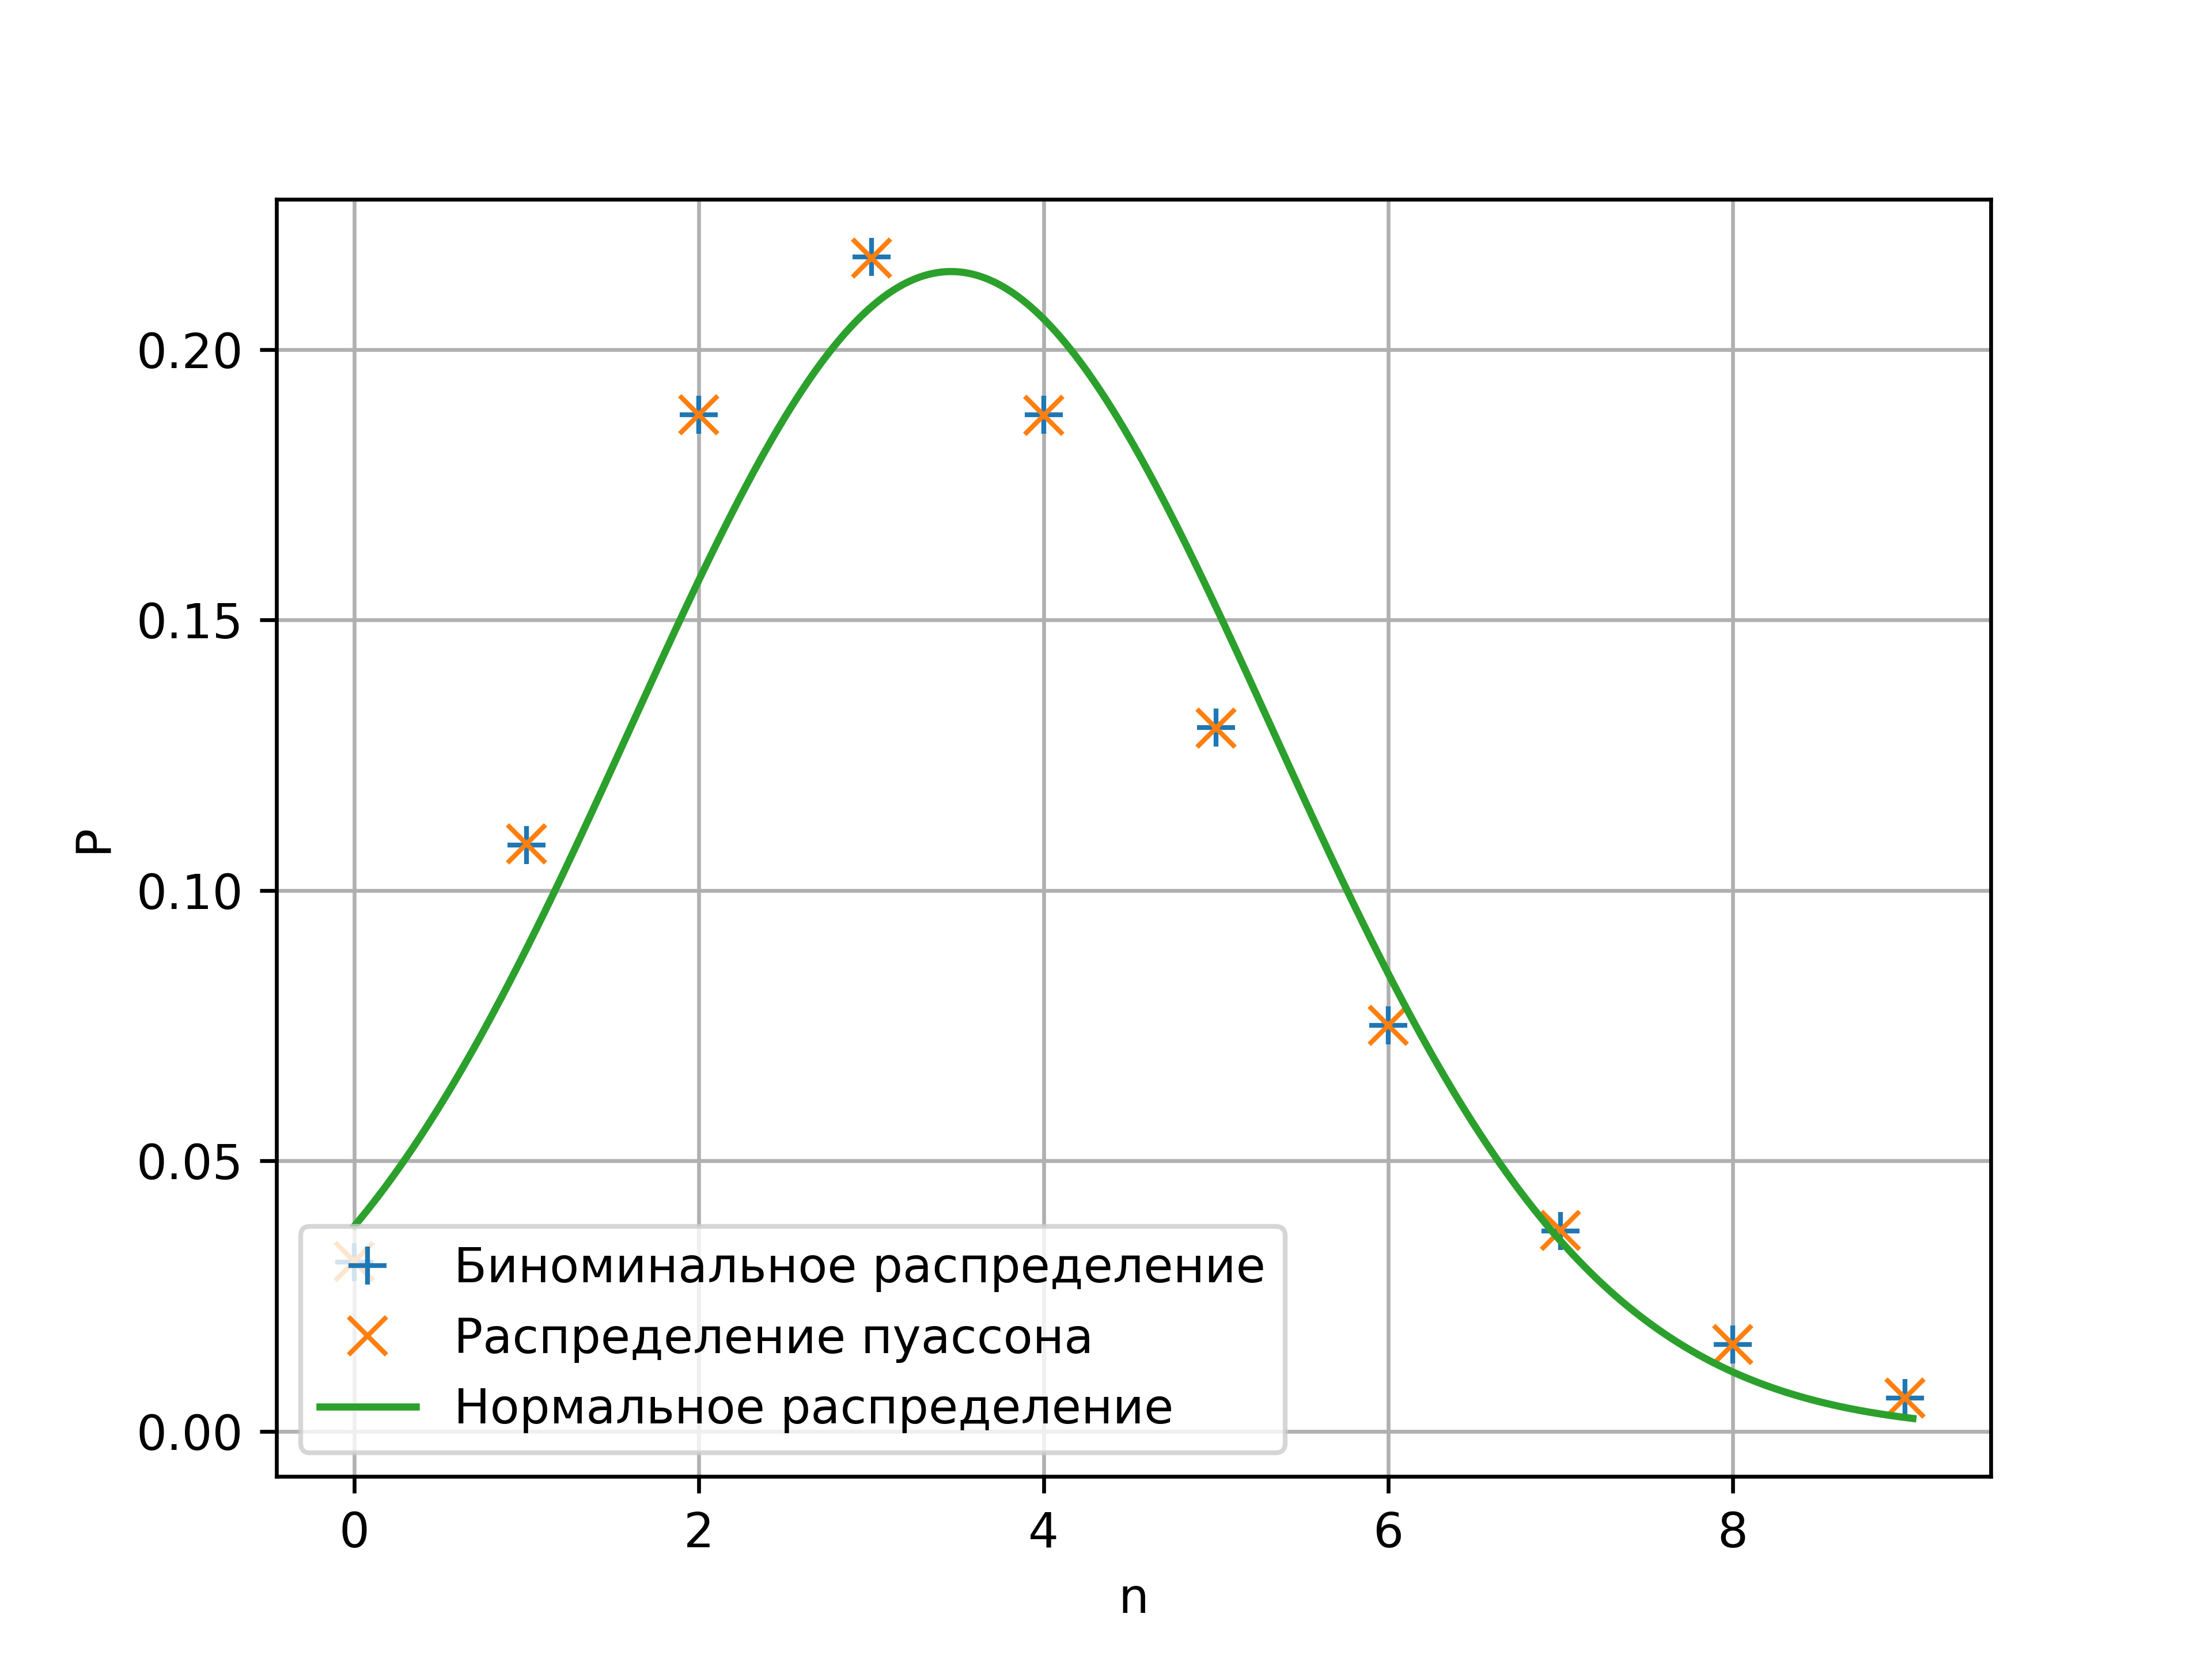
\includegraphics[width=0.49\linewidth]{raspr.png}
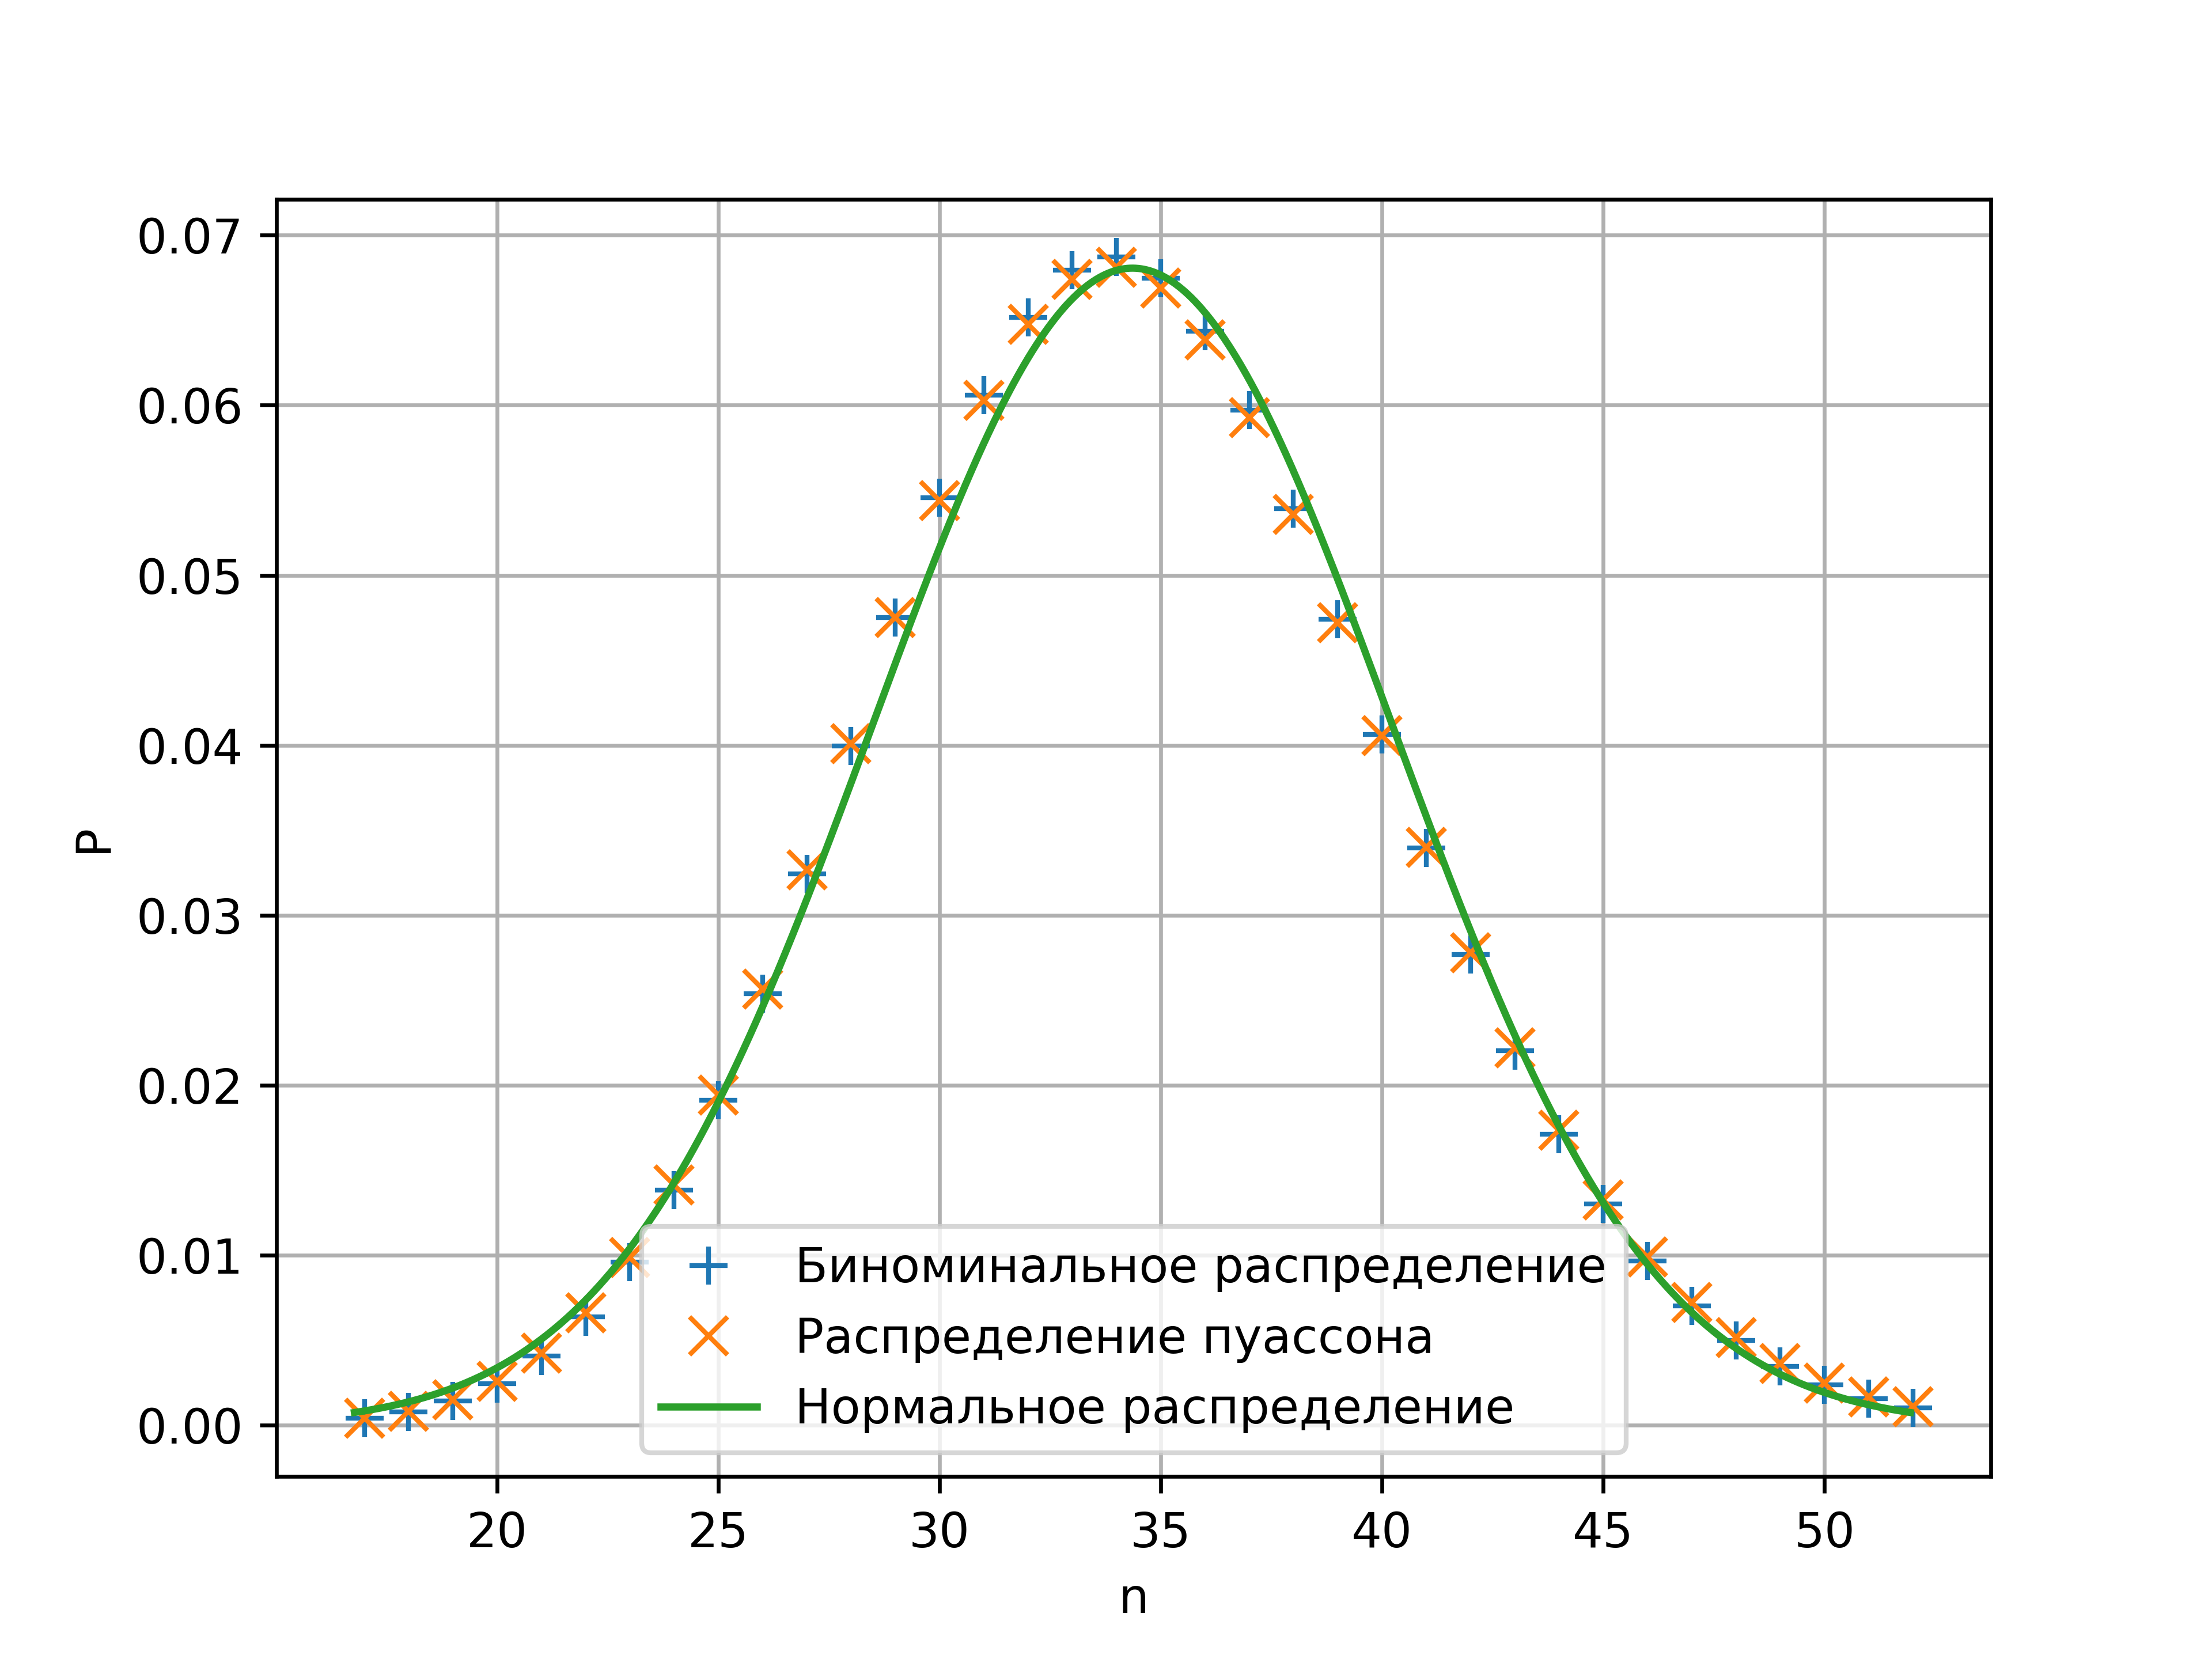
\includegraphics[width=0.49\linewidth]{raspr2.png}
\caption{Распределения на разных масштабах.}
\label{fig:rasp1}
\end{figure}







\section {Экспериментальная установка}
Установка состоит из сцинтиллятора, фооэлектронного умножителя, пересчетного устройства и компьютера.
Принцип работы: $\alpha$-частица, попадая в сцинтиллятор порождает вспышку света. Внутри ФЭУ в вакууму расположены металлические пластины с
маленькой работой выхода. Фотон выбивает электрон из такой пластины, электрон разгоняется электрическим полем, попадает на следующую пластину и выбивает
несколько электронов, которые выбивают из следующей пластины еще больше электронов и.т.д. Пересчетное устройство регистрирует увеличение силы тока, потребляемого ФЭУ в момент
попадания $\alpha$-частицы. Чем большую энергию имеет $\alpha$-частица, тем больше электронов она выбивает, тем больший ток потребляет ФЭУ.




\section {Проведение измерений}

Внутри ФЭУ электроны из-за теплового движения могут вылетать под действием электрического поля. Для компенсации этого эффекта
был выбран порог энергии для регистрации $\alpha$-частицы. Также были проведены измерения без образца в детекторе.

\begin{figure}[H]
\centering
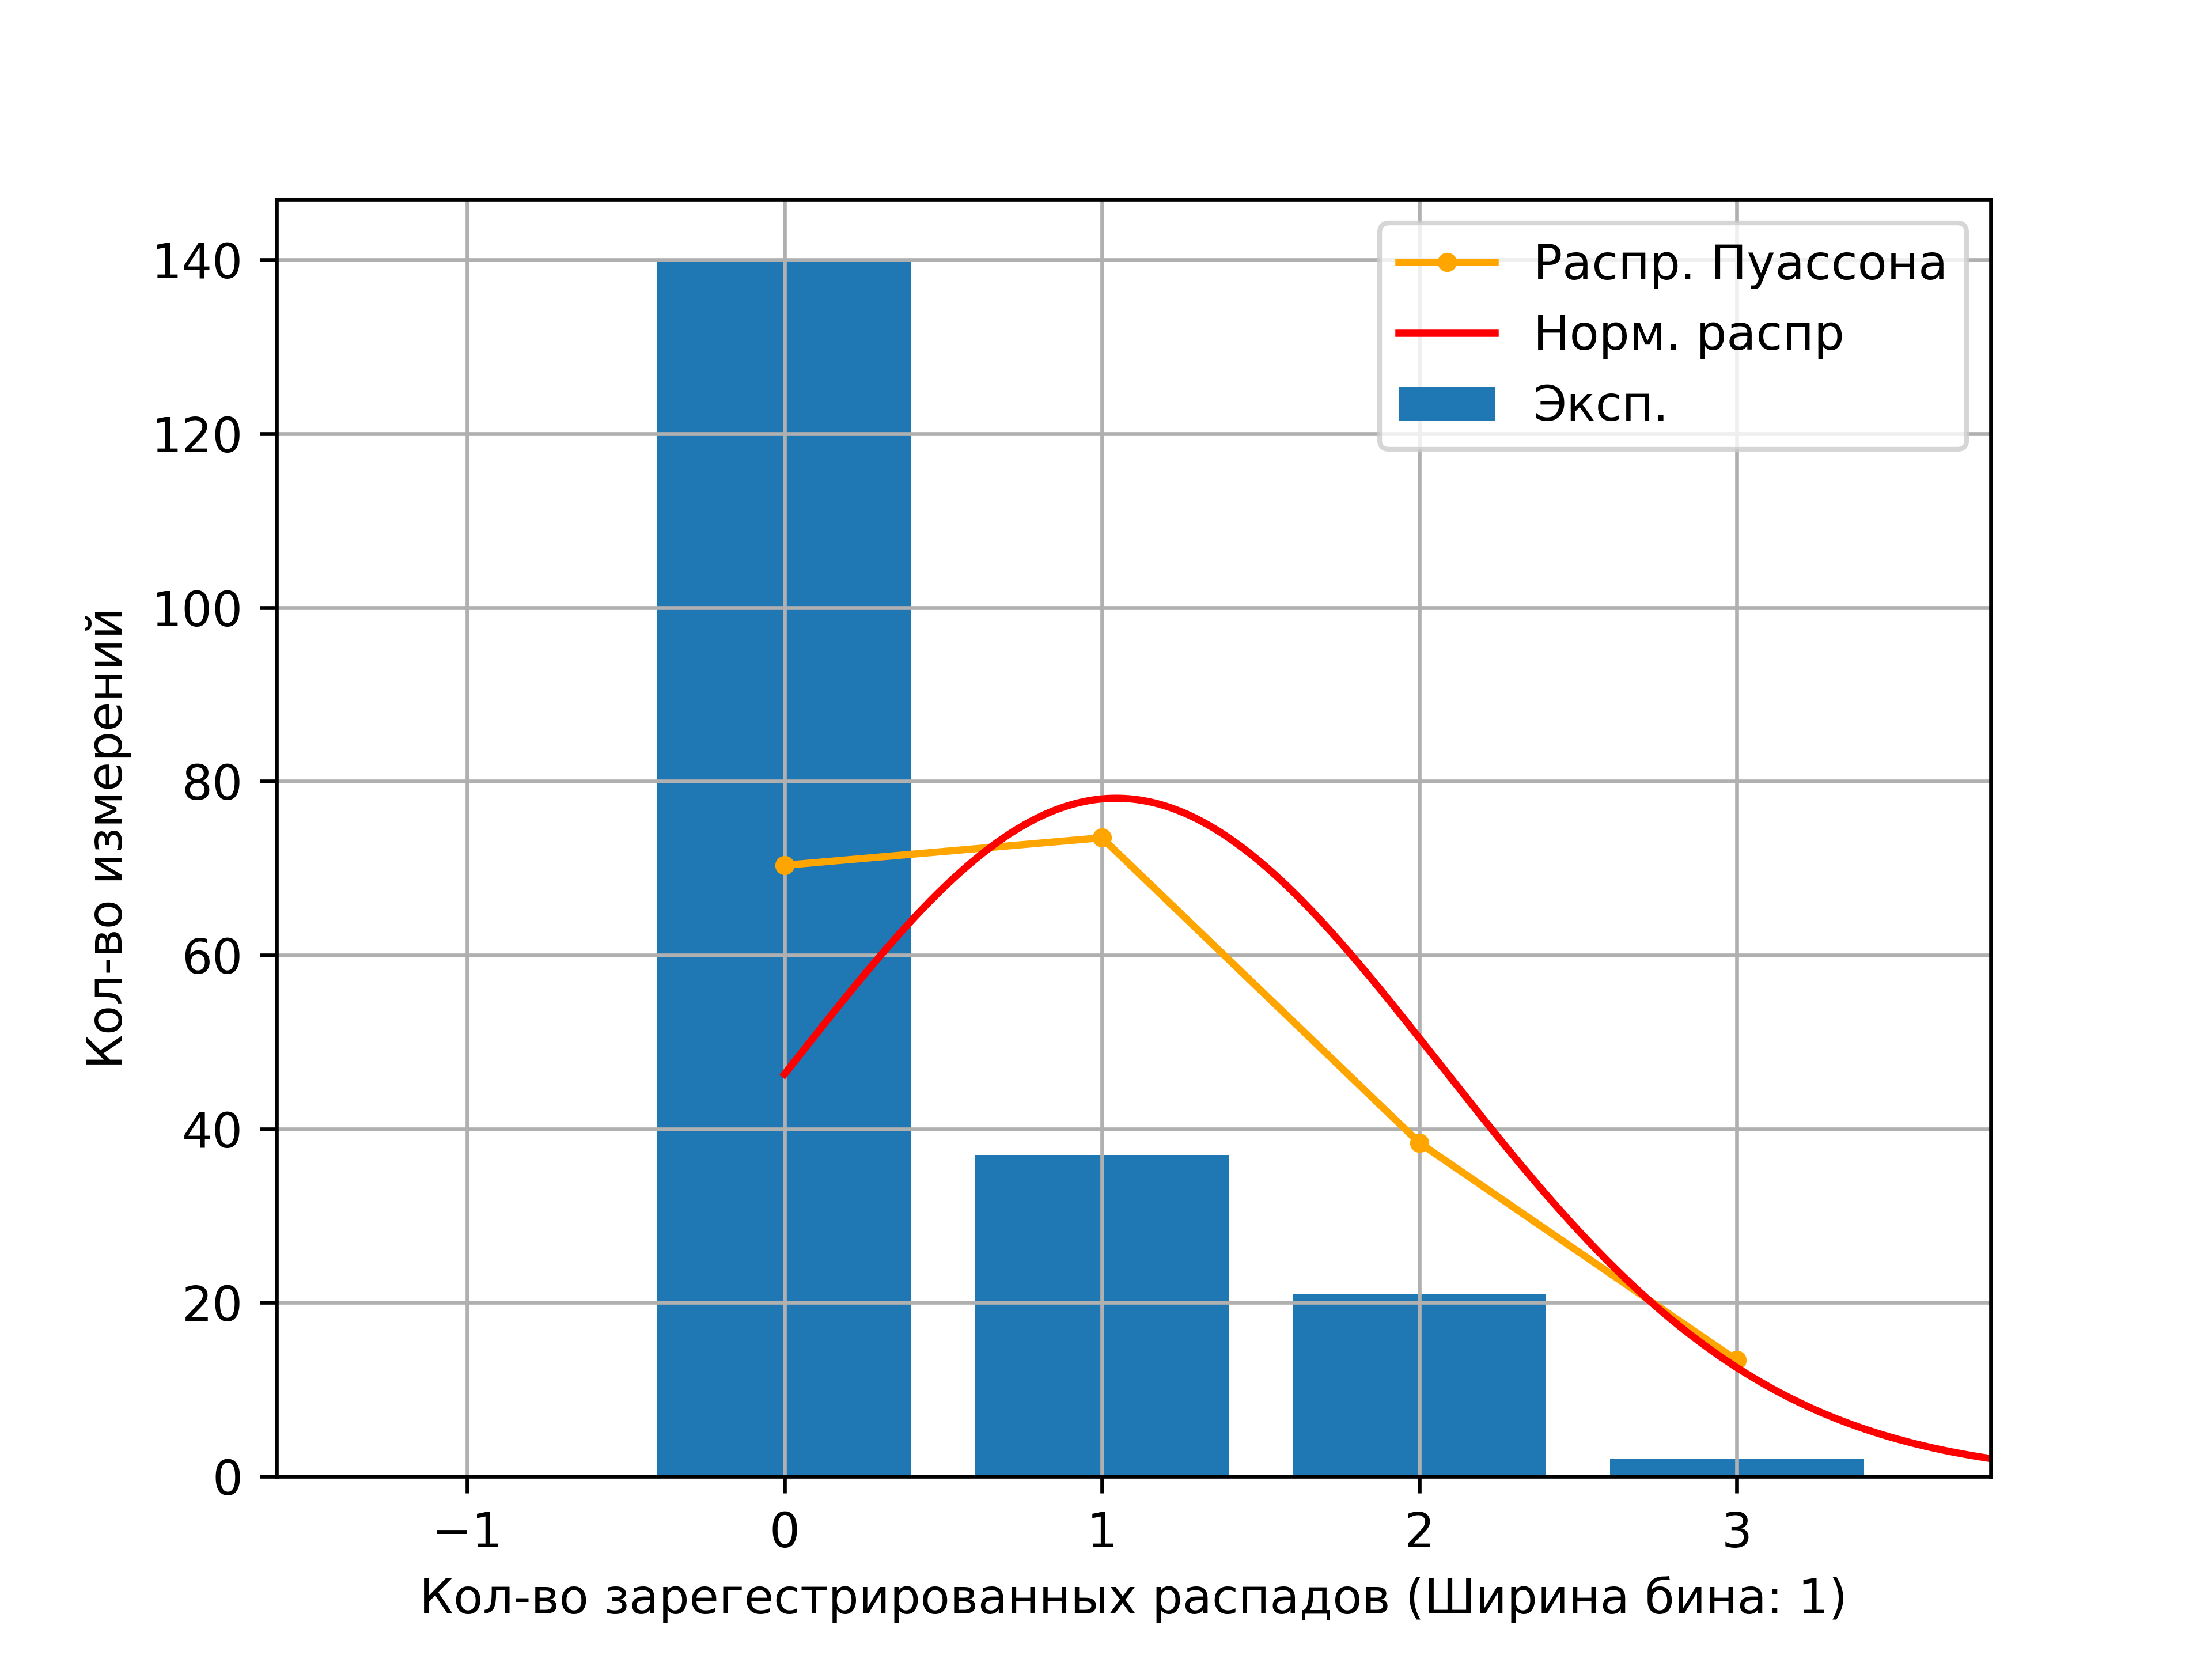
\includegraphics[width=0.5\linewidth]{dt1000_n200_no_Pu.png}
\caption{Распределение без образца в детекторе (t = 1000мс, N = 200)}
\label{fig:no_pu}
\end{figure}


Были проведены ряды измерений, для построения зависимости неопределенности среднего числа распадов от количества
выборок и от времени экспозиции каждой выборки:



\begin{figure}[H]
\centering
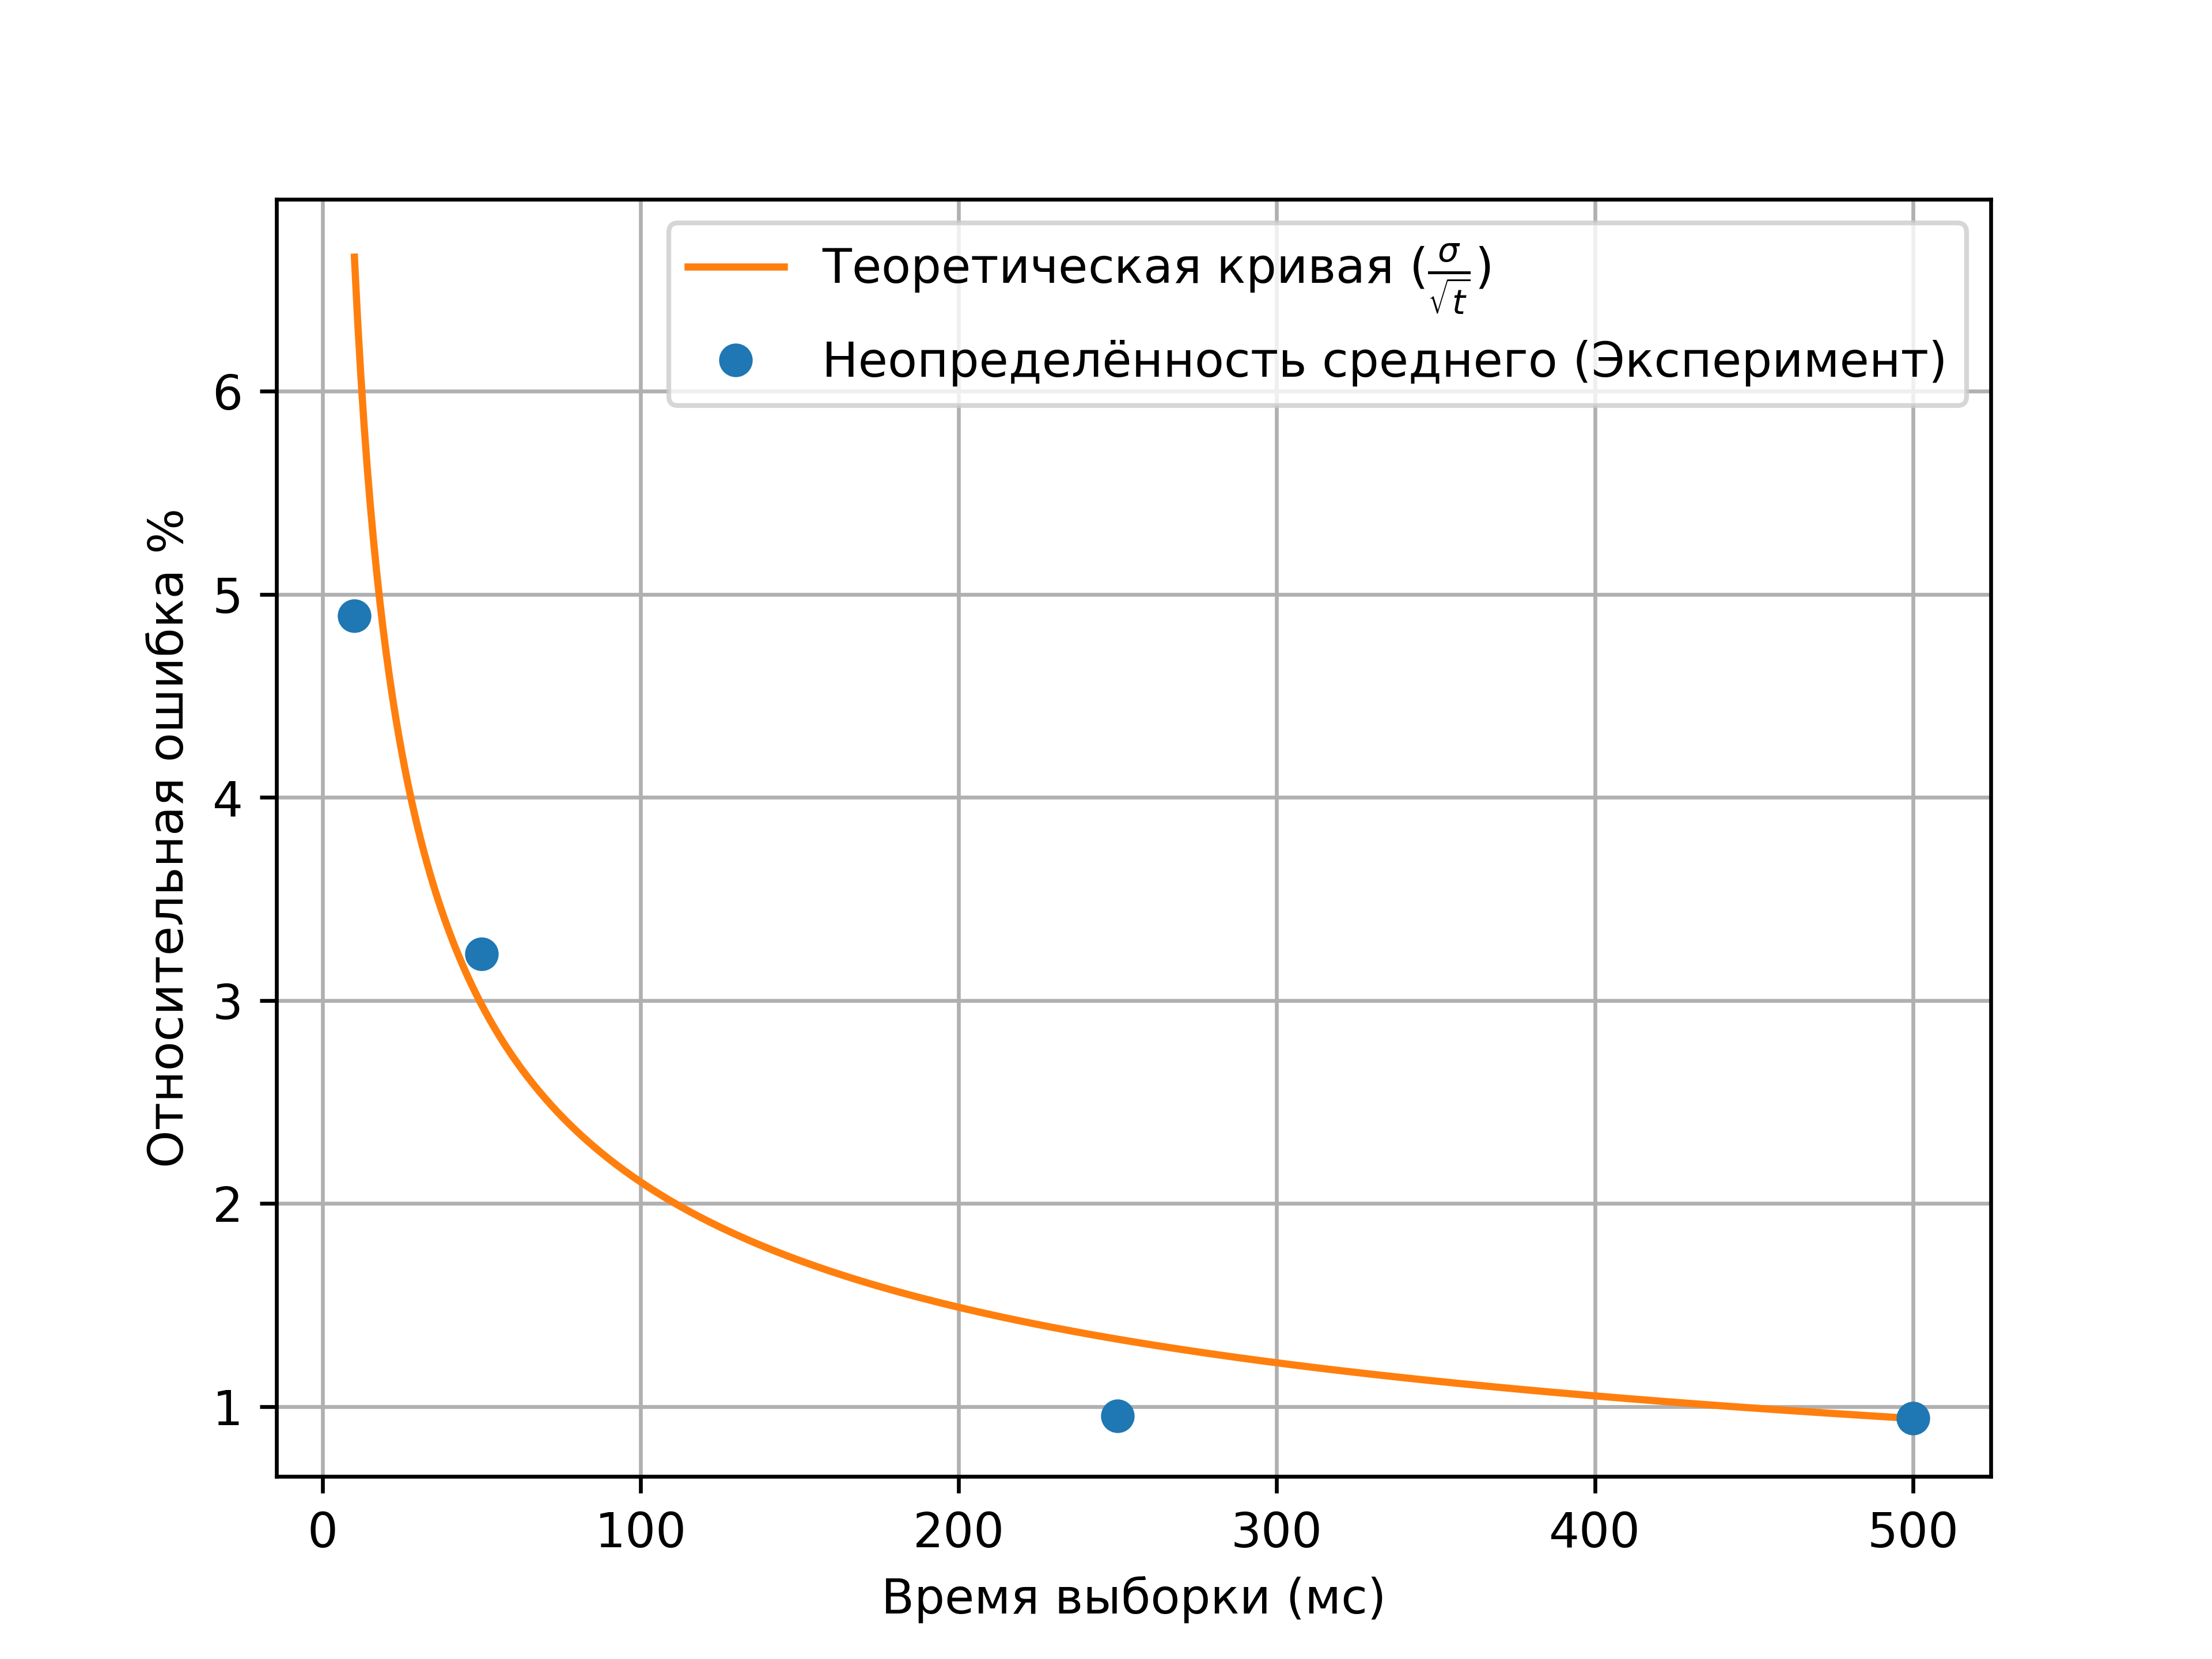
\includegraphics[width=0.5\linewidth]{Error_dt.png}
\caption{Относительная неопределенность измерений при изменении времени экспозиции}
\label{fig:errordt}
\end{figure}

\begin{figure}[H]
\centering
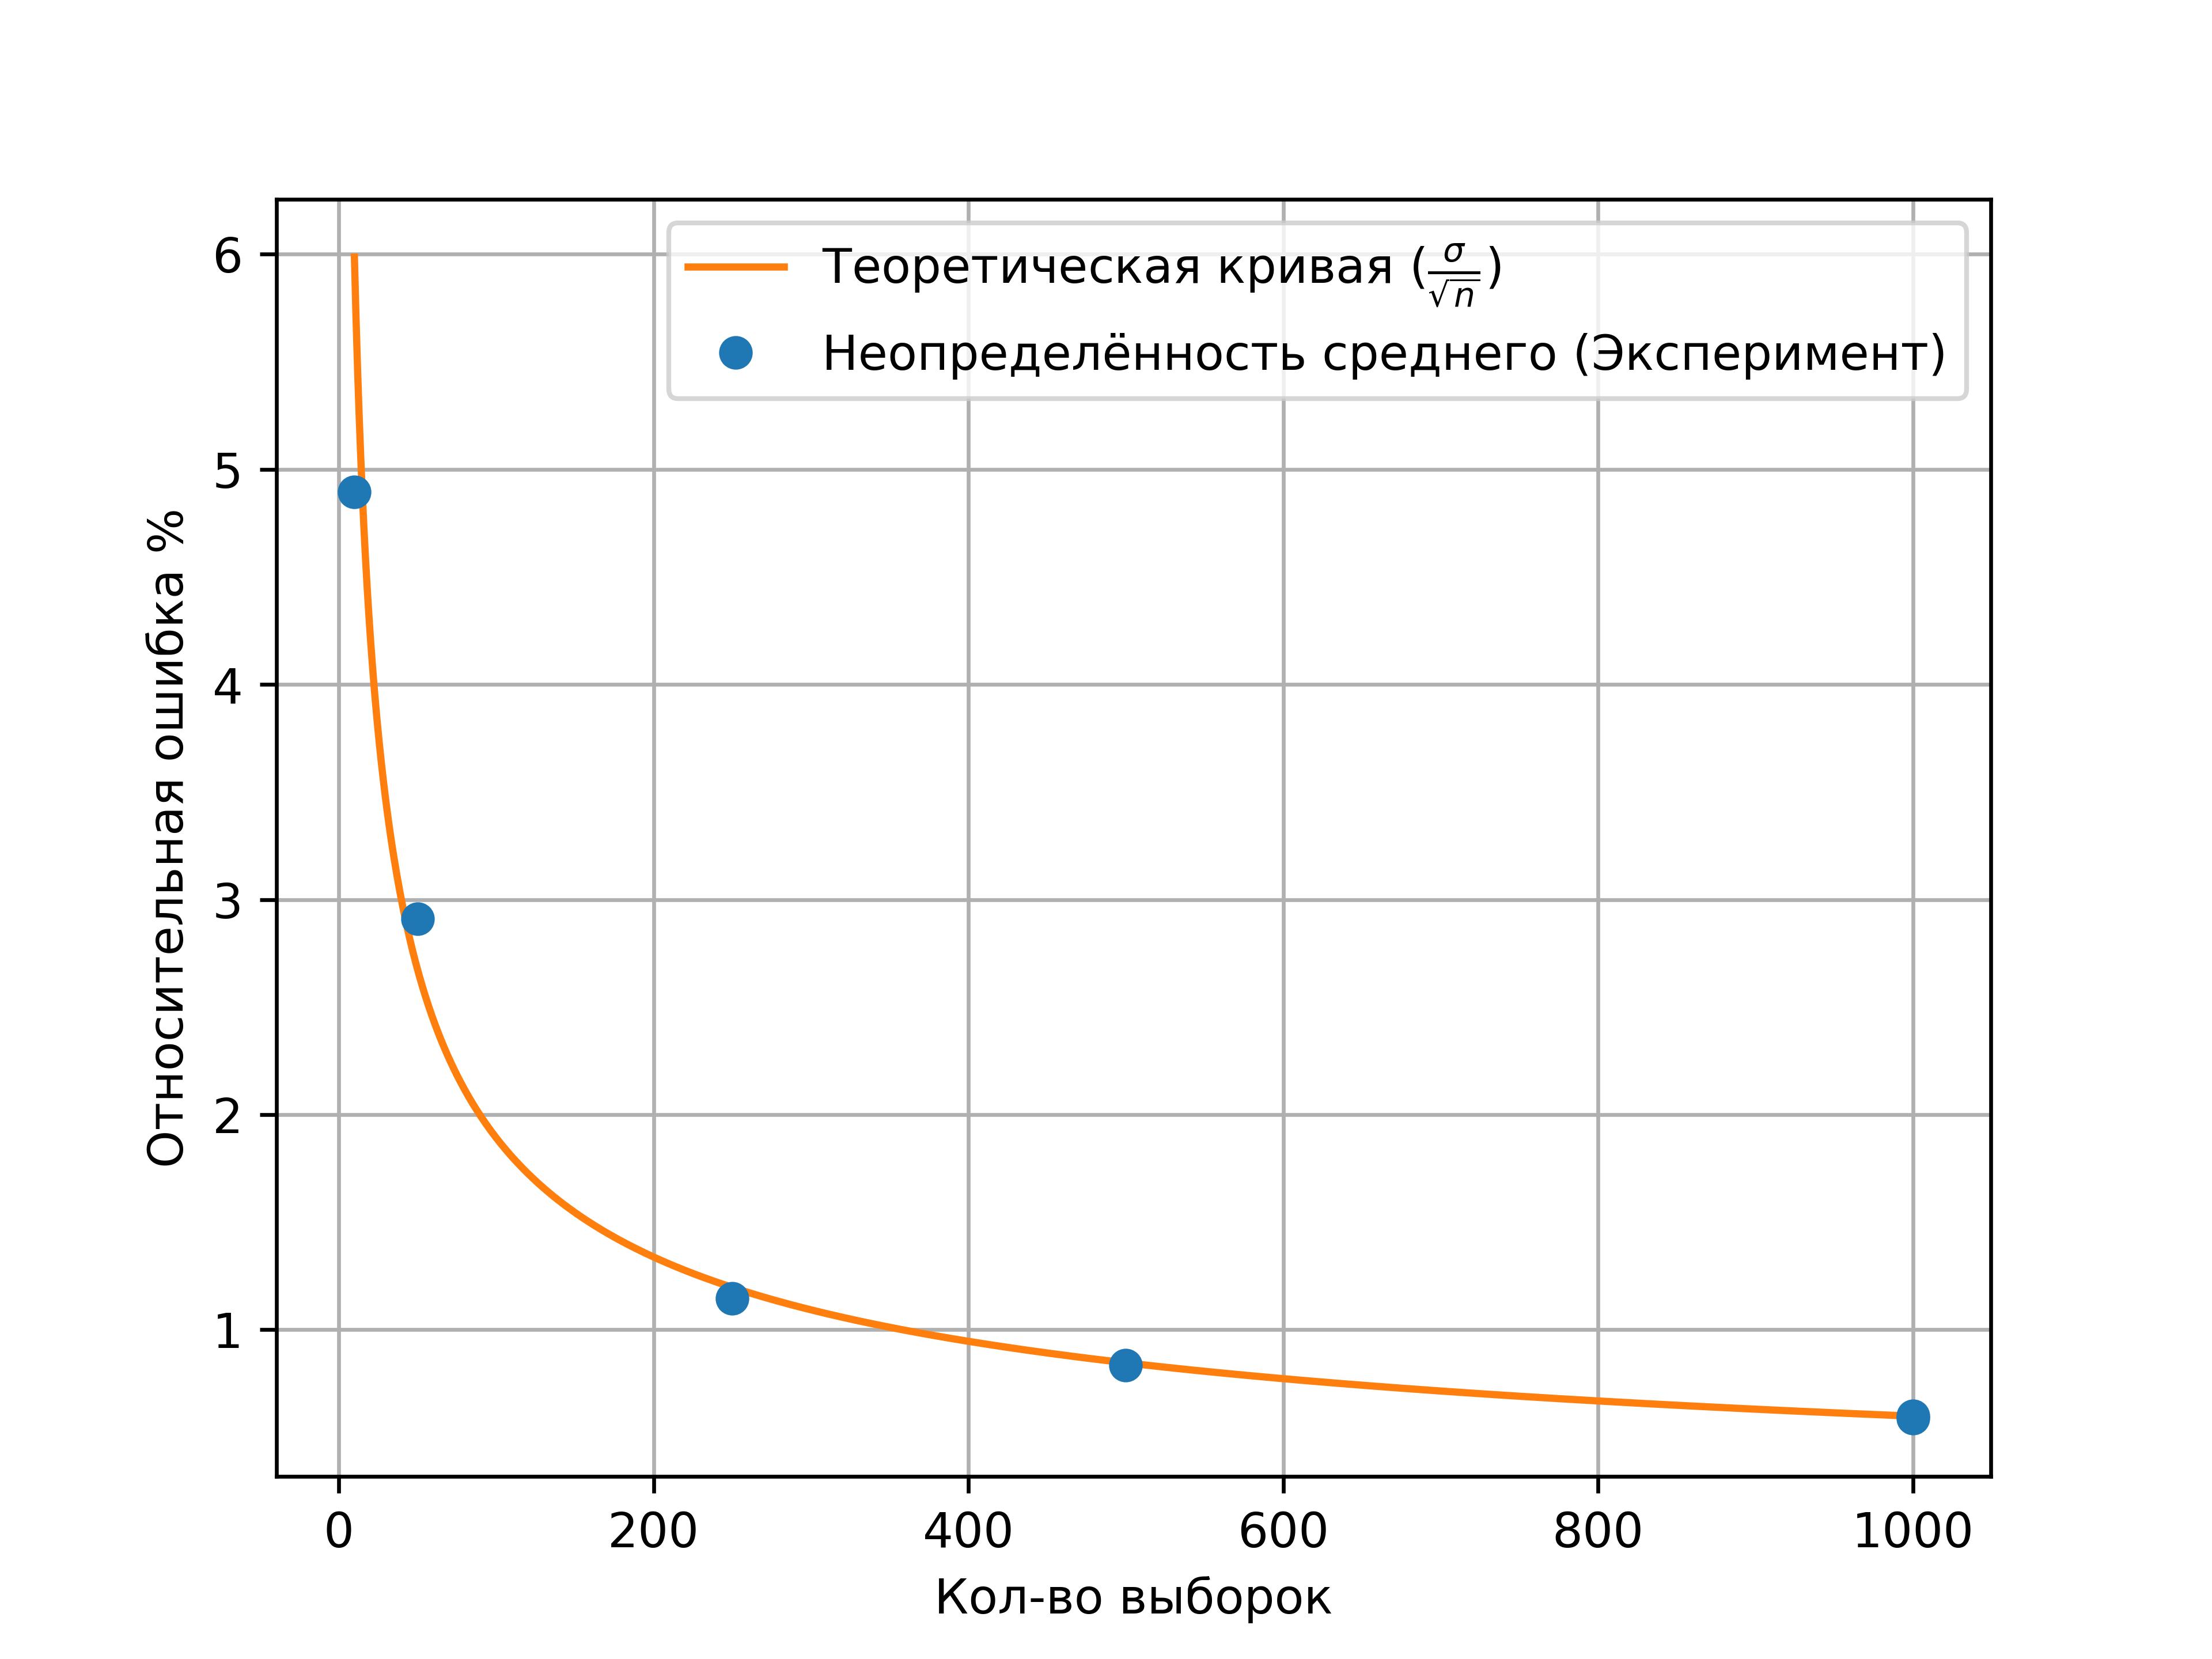
\includegraphics[width=0.5\linewidth]{Error_n.png}
\caption{Относительная неопределенность измерений при изменении числа выборок}
\label{fig:errorn}
\end{figure}



\section{Результаты измерений}

\begin{figure}[H]
\centering

\includegraphics[width=0.5\linewidth]{QR.png}
\caption{Ссылка на исходные данные измерений}
\label{fig:QR}
\end{figure}


\begin{figure}[H]
\centering
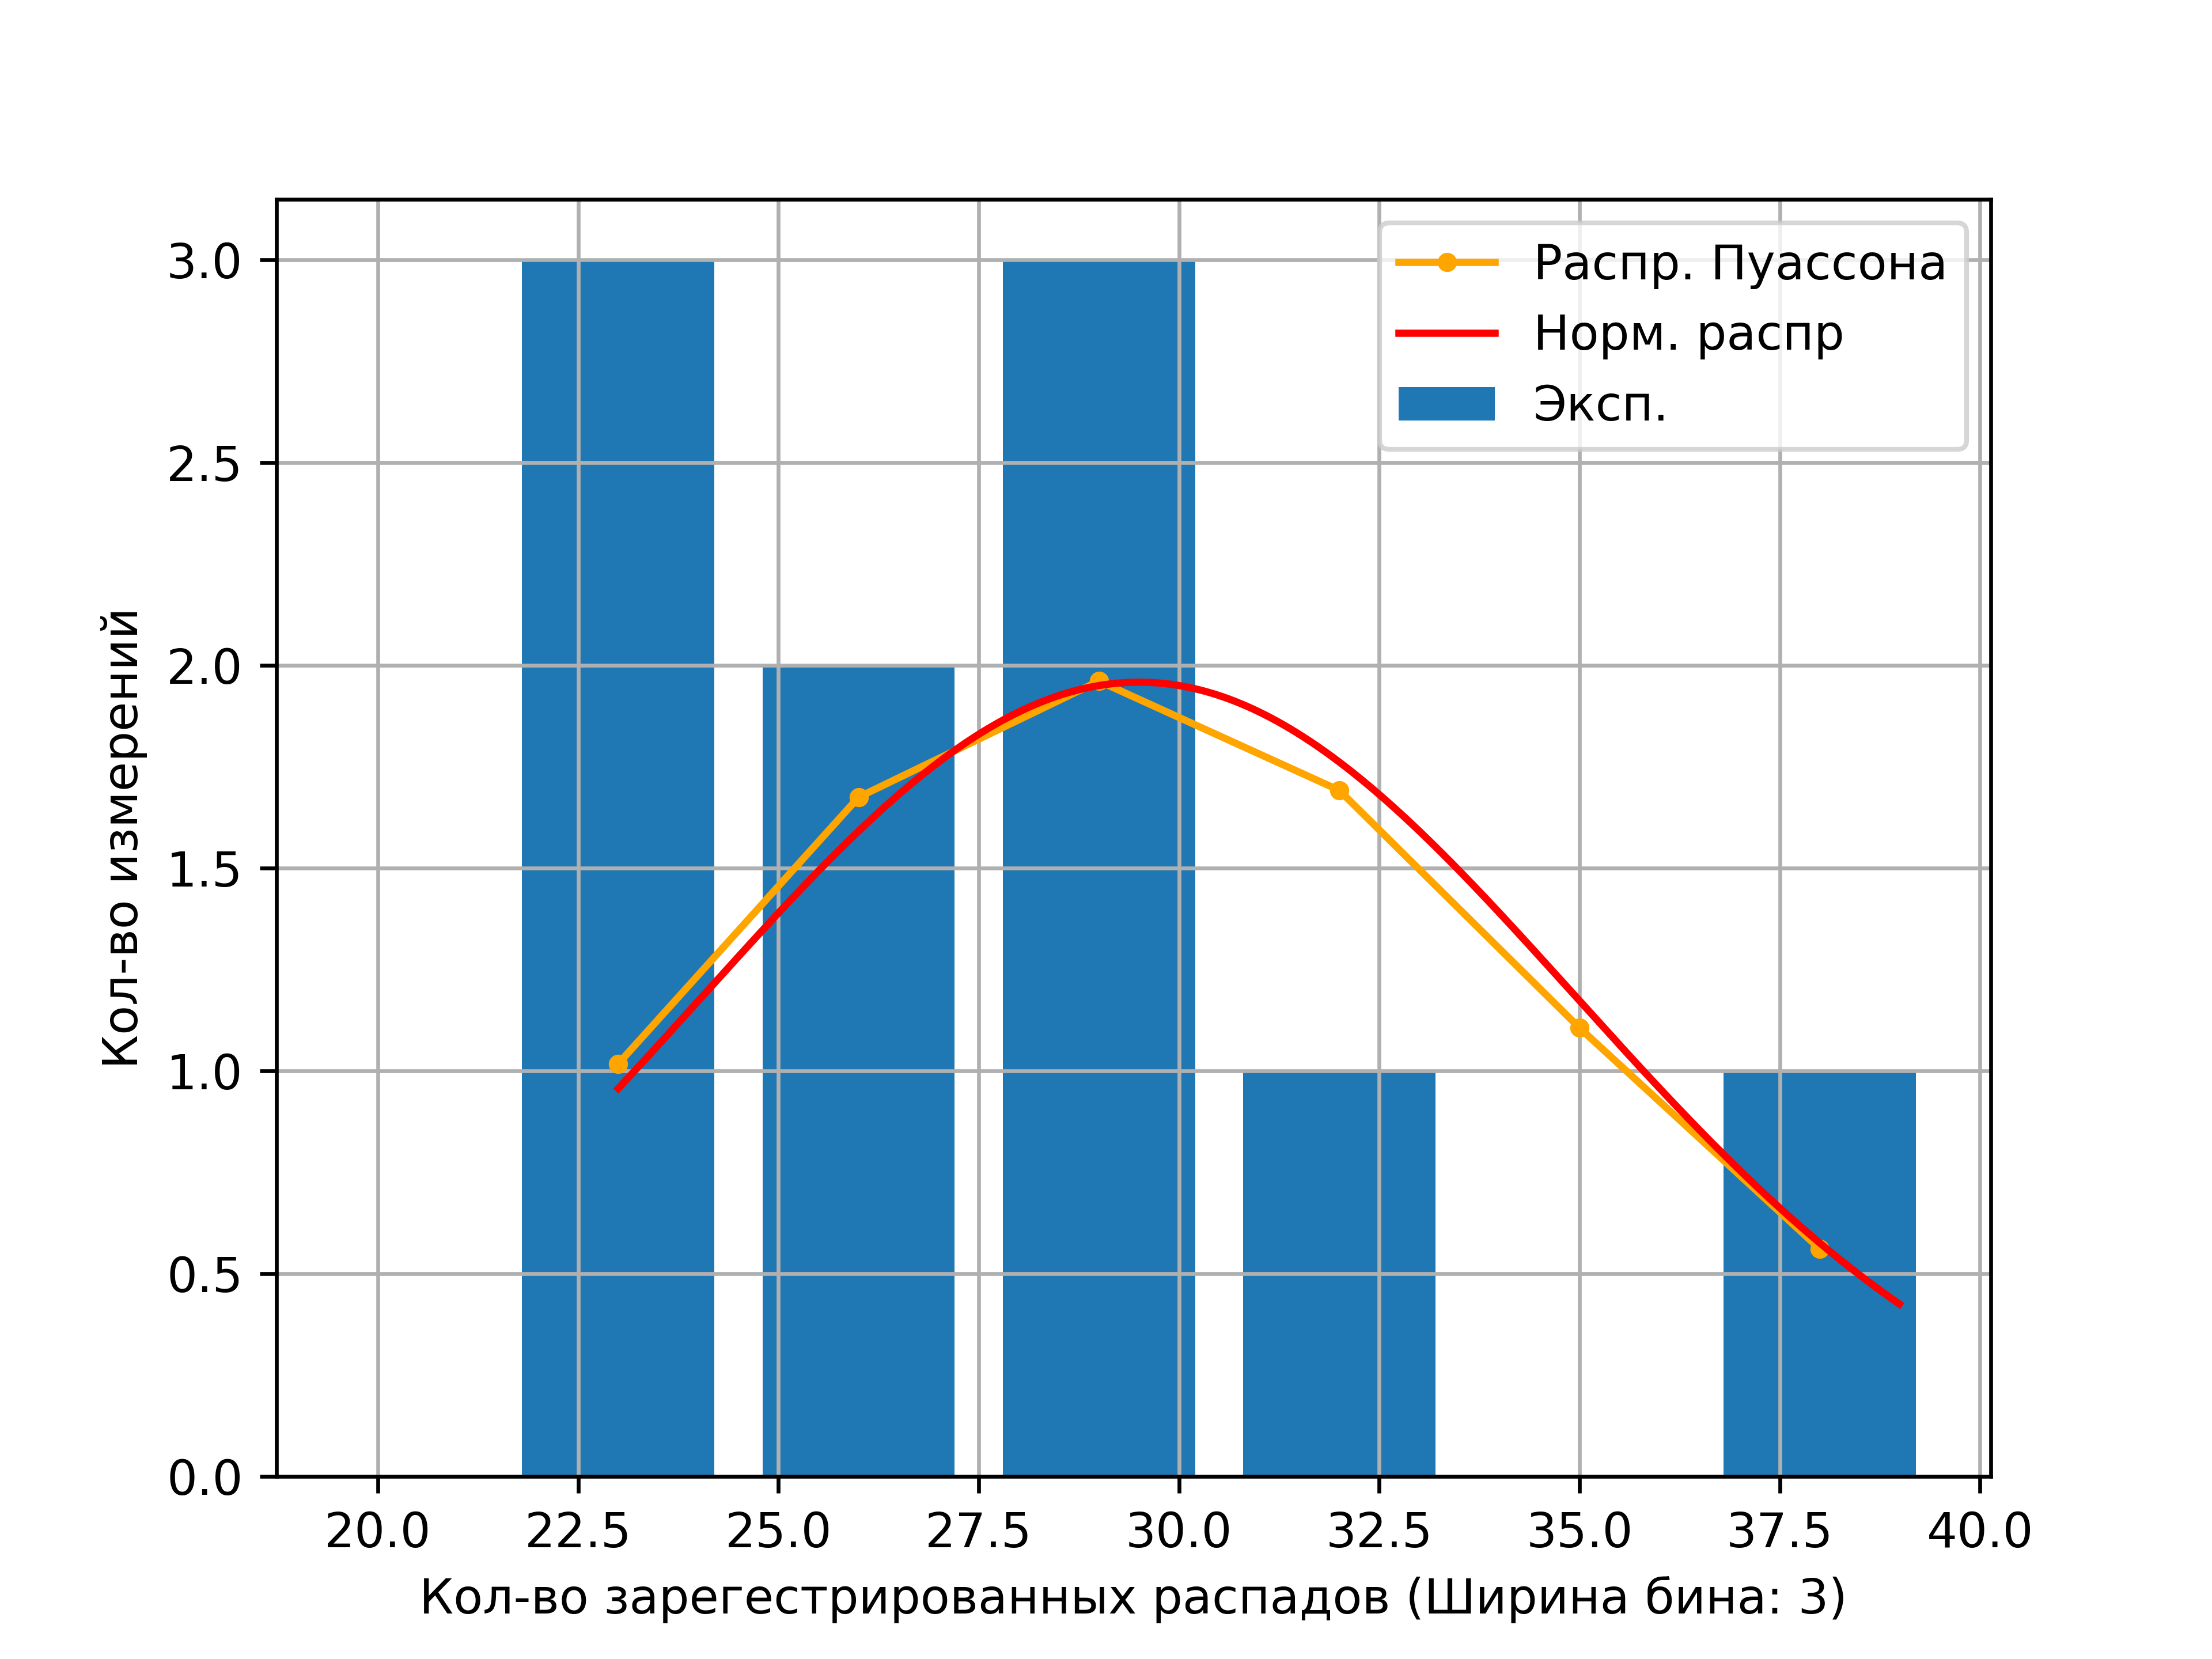
\includegraphics[width=0.5\linewidth]{dt10_n10.png}
\caption{10 выборок по 10 мс}
\label{fig:dt10n10}
\end{figure}

\begin{figure}[H]
\centering
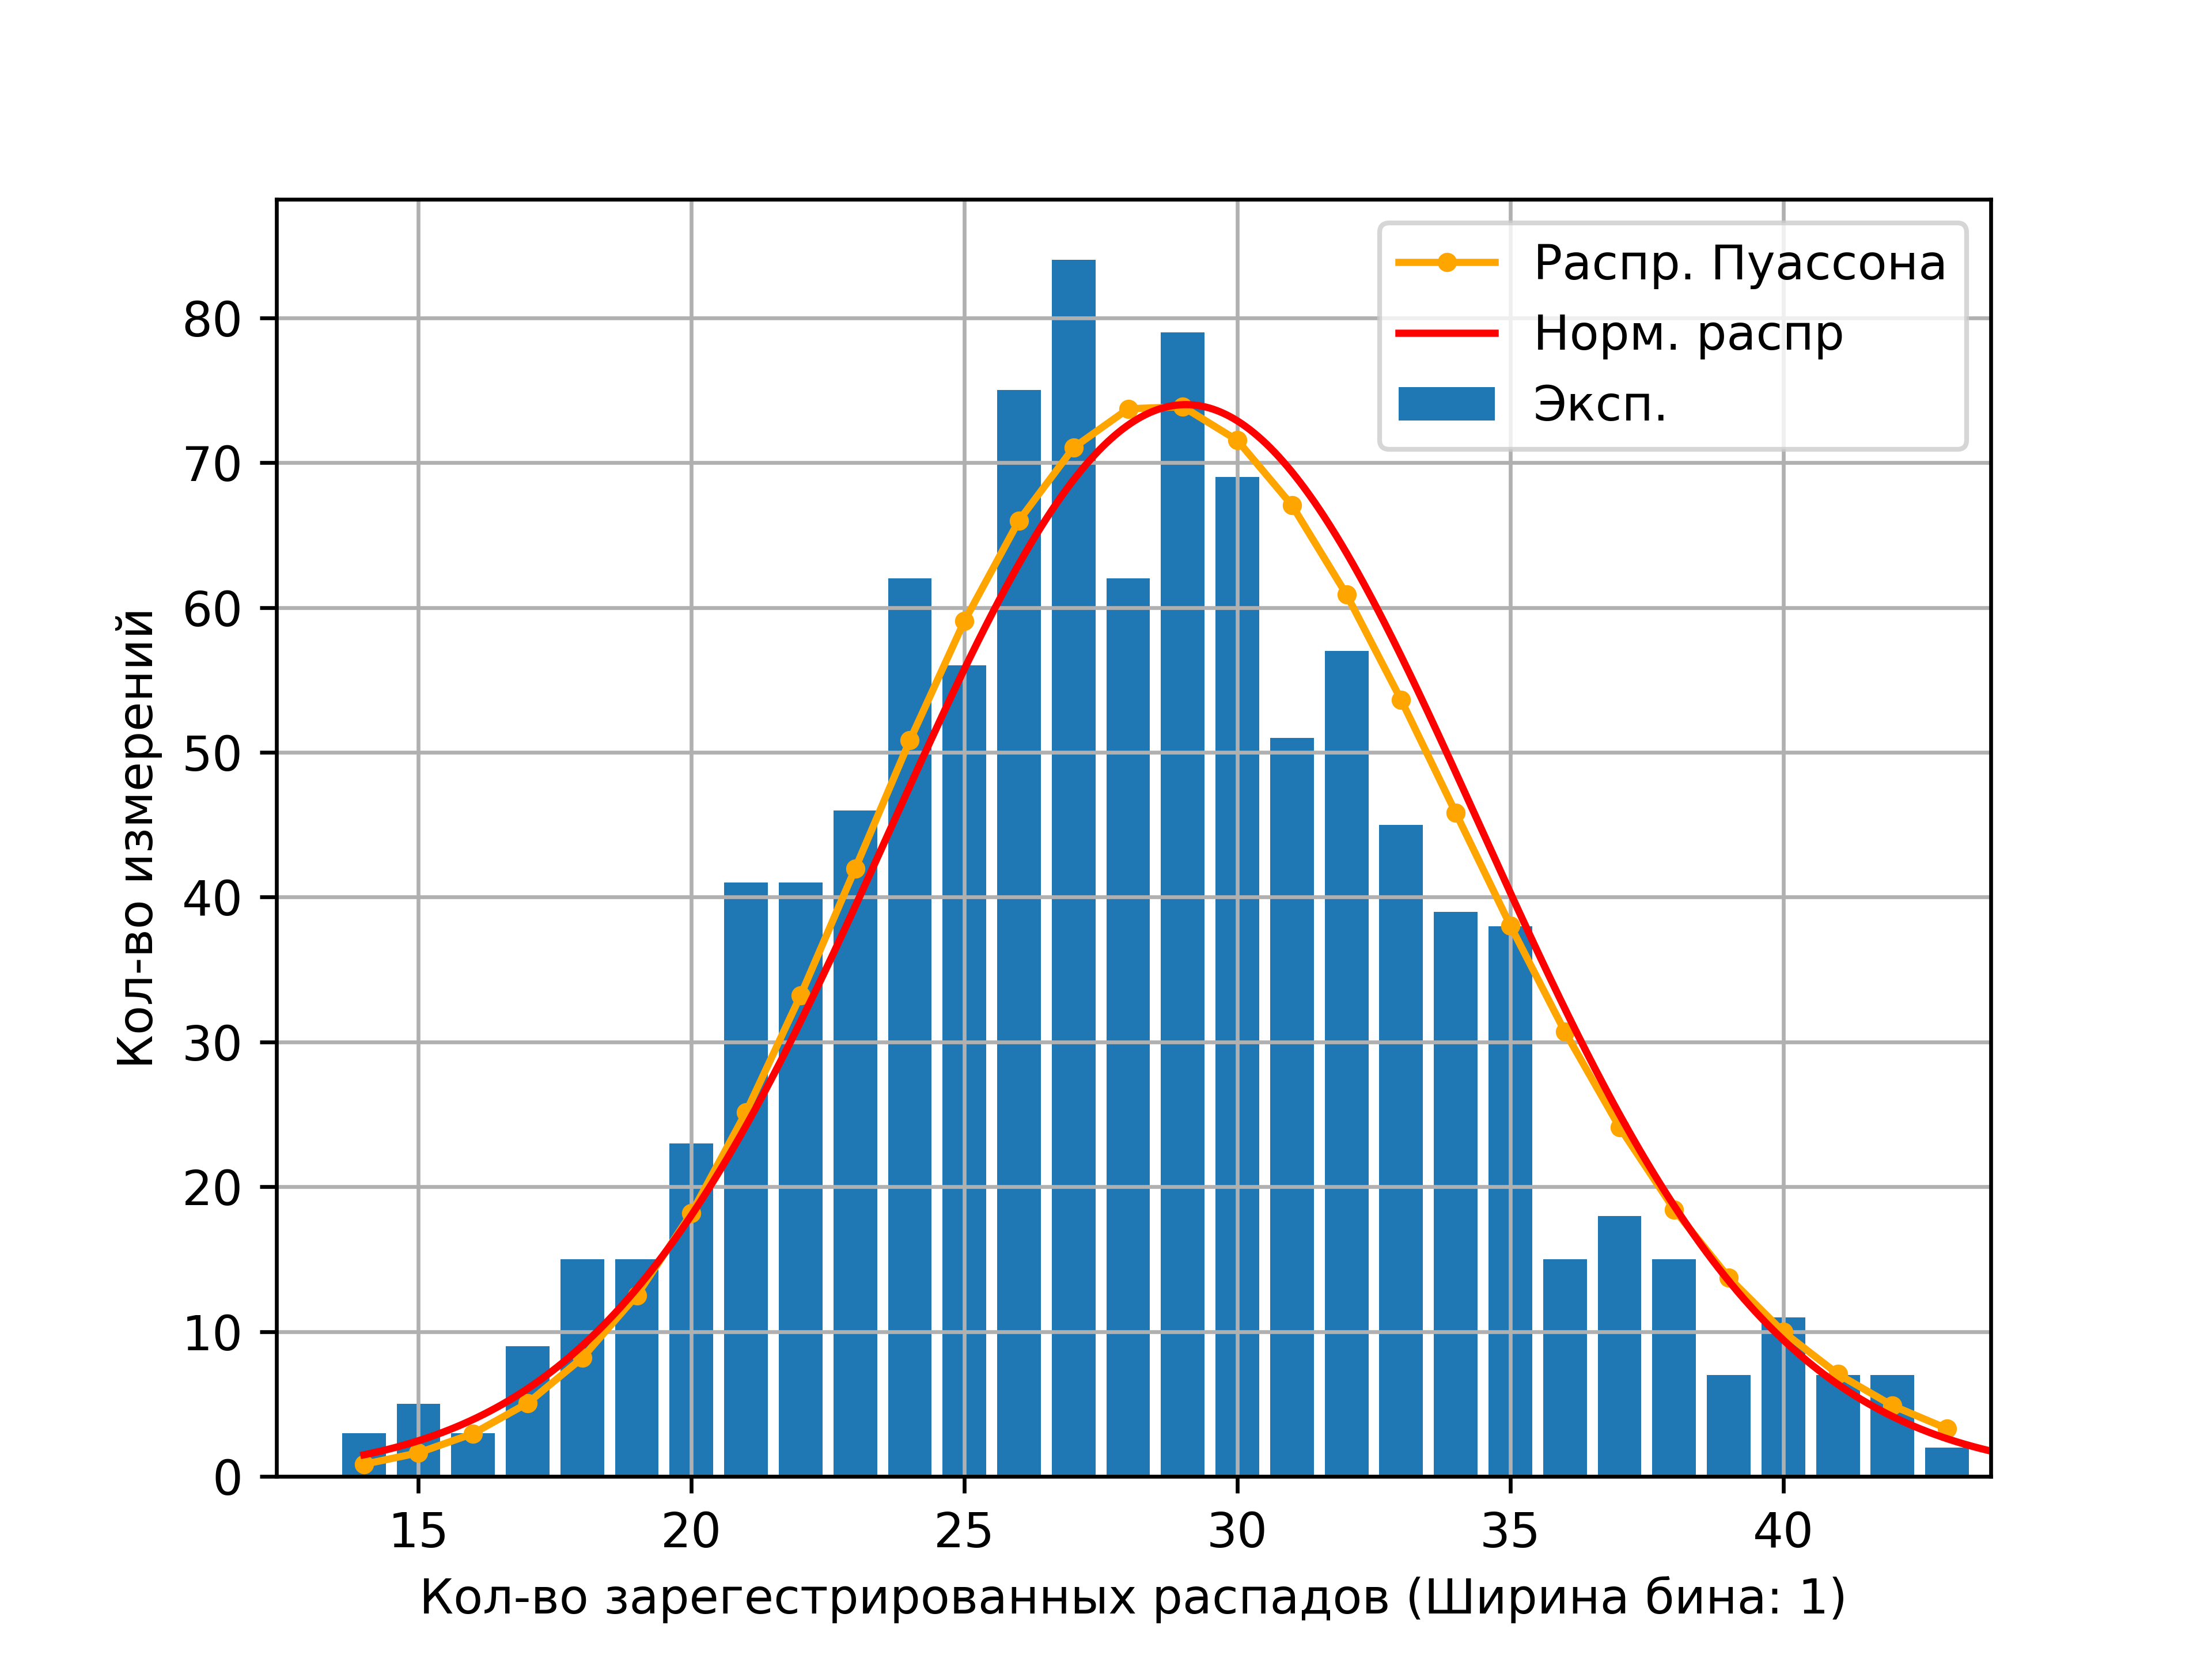
\includegraphics[width=0.5\linewidth]{dt10_n1000.png}
\caption{1000 выборок по 10 мс}
\label{fig:dt10n10000}
\end{figure}



\begin{figure}[H]
\centering
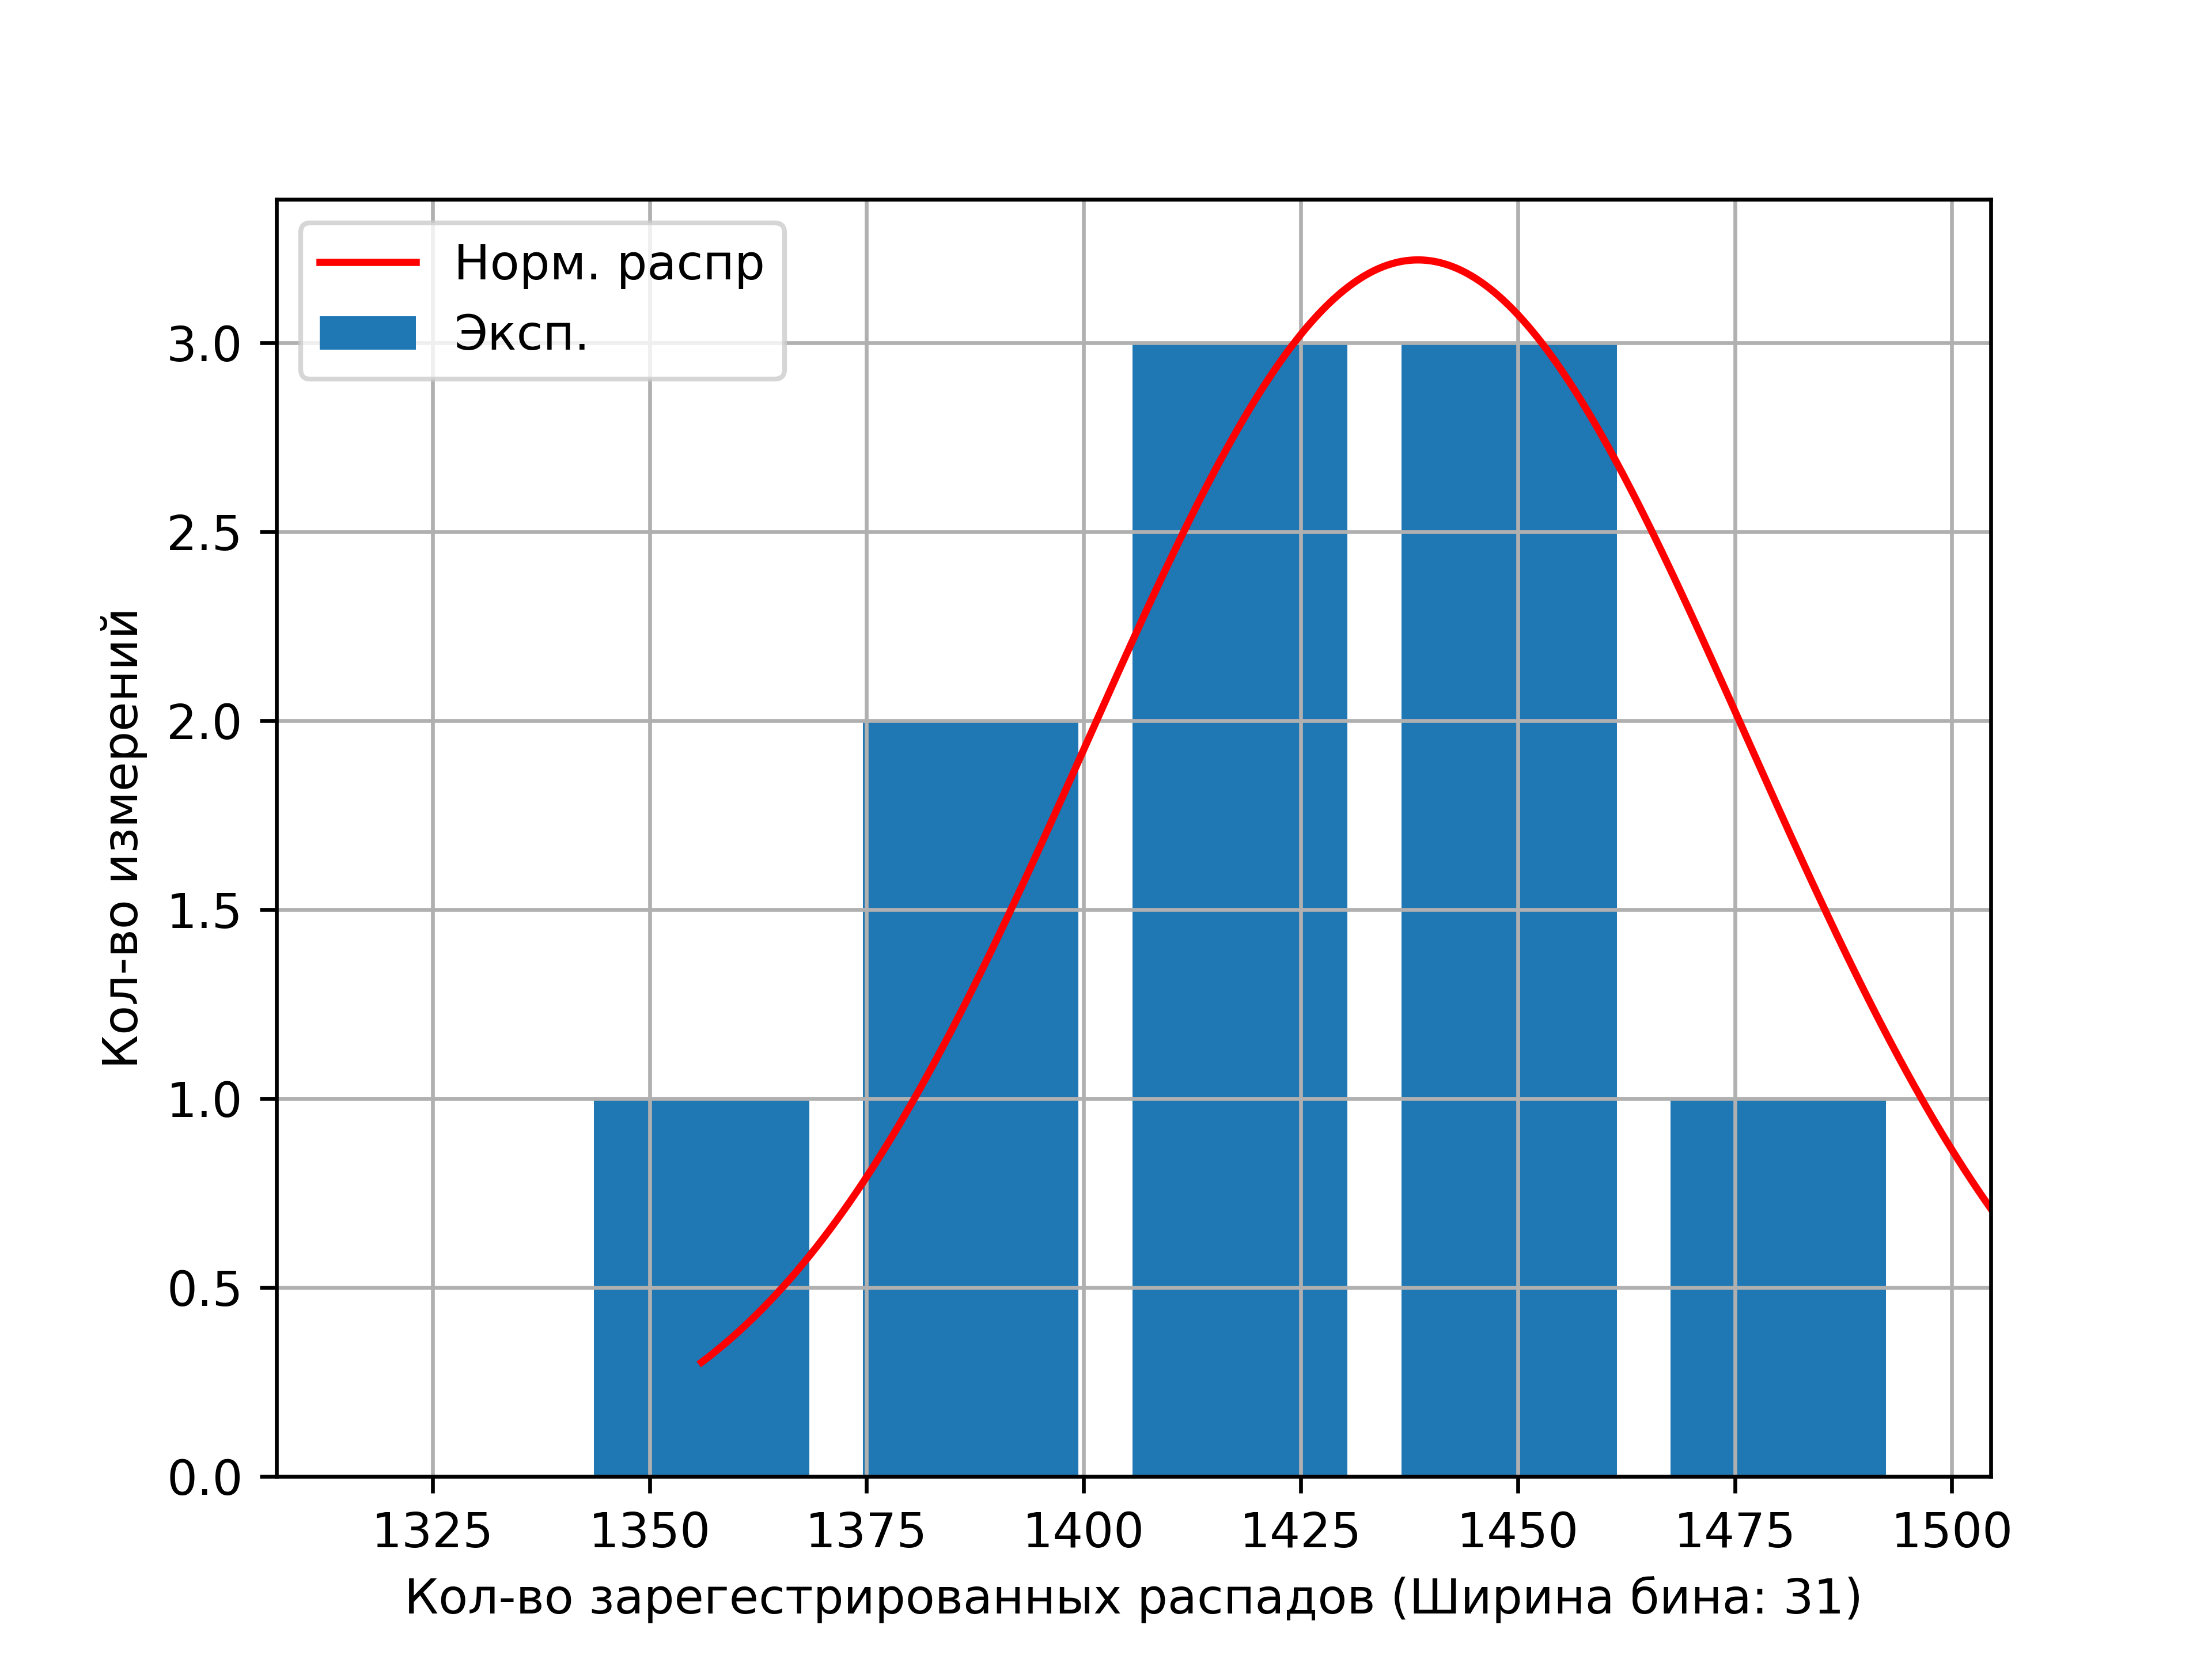
\includegraphics[width=0.5\linewidth]{dt500_n10.png}
\caption{10 выборок по 500 мс}
\label{fig:dt500n10}
\end{figure}


\begin{figure}[H]
\centering
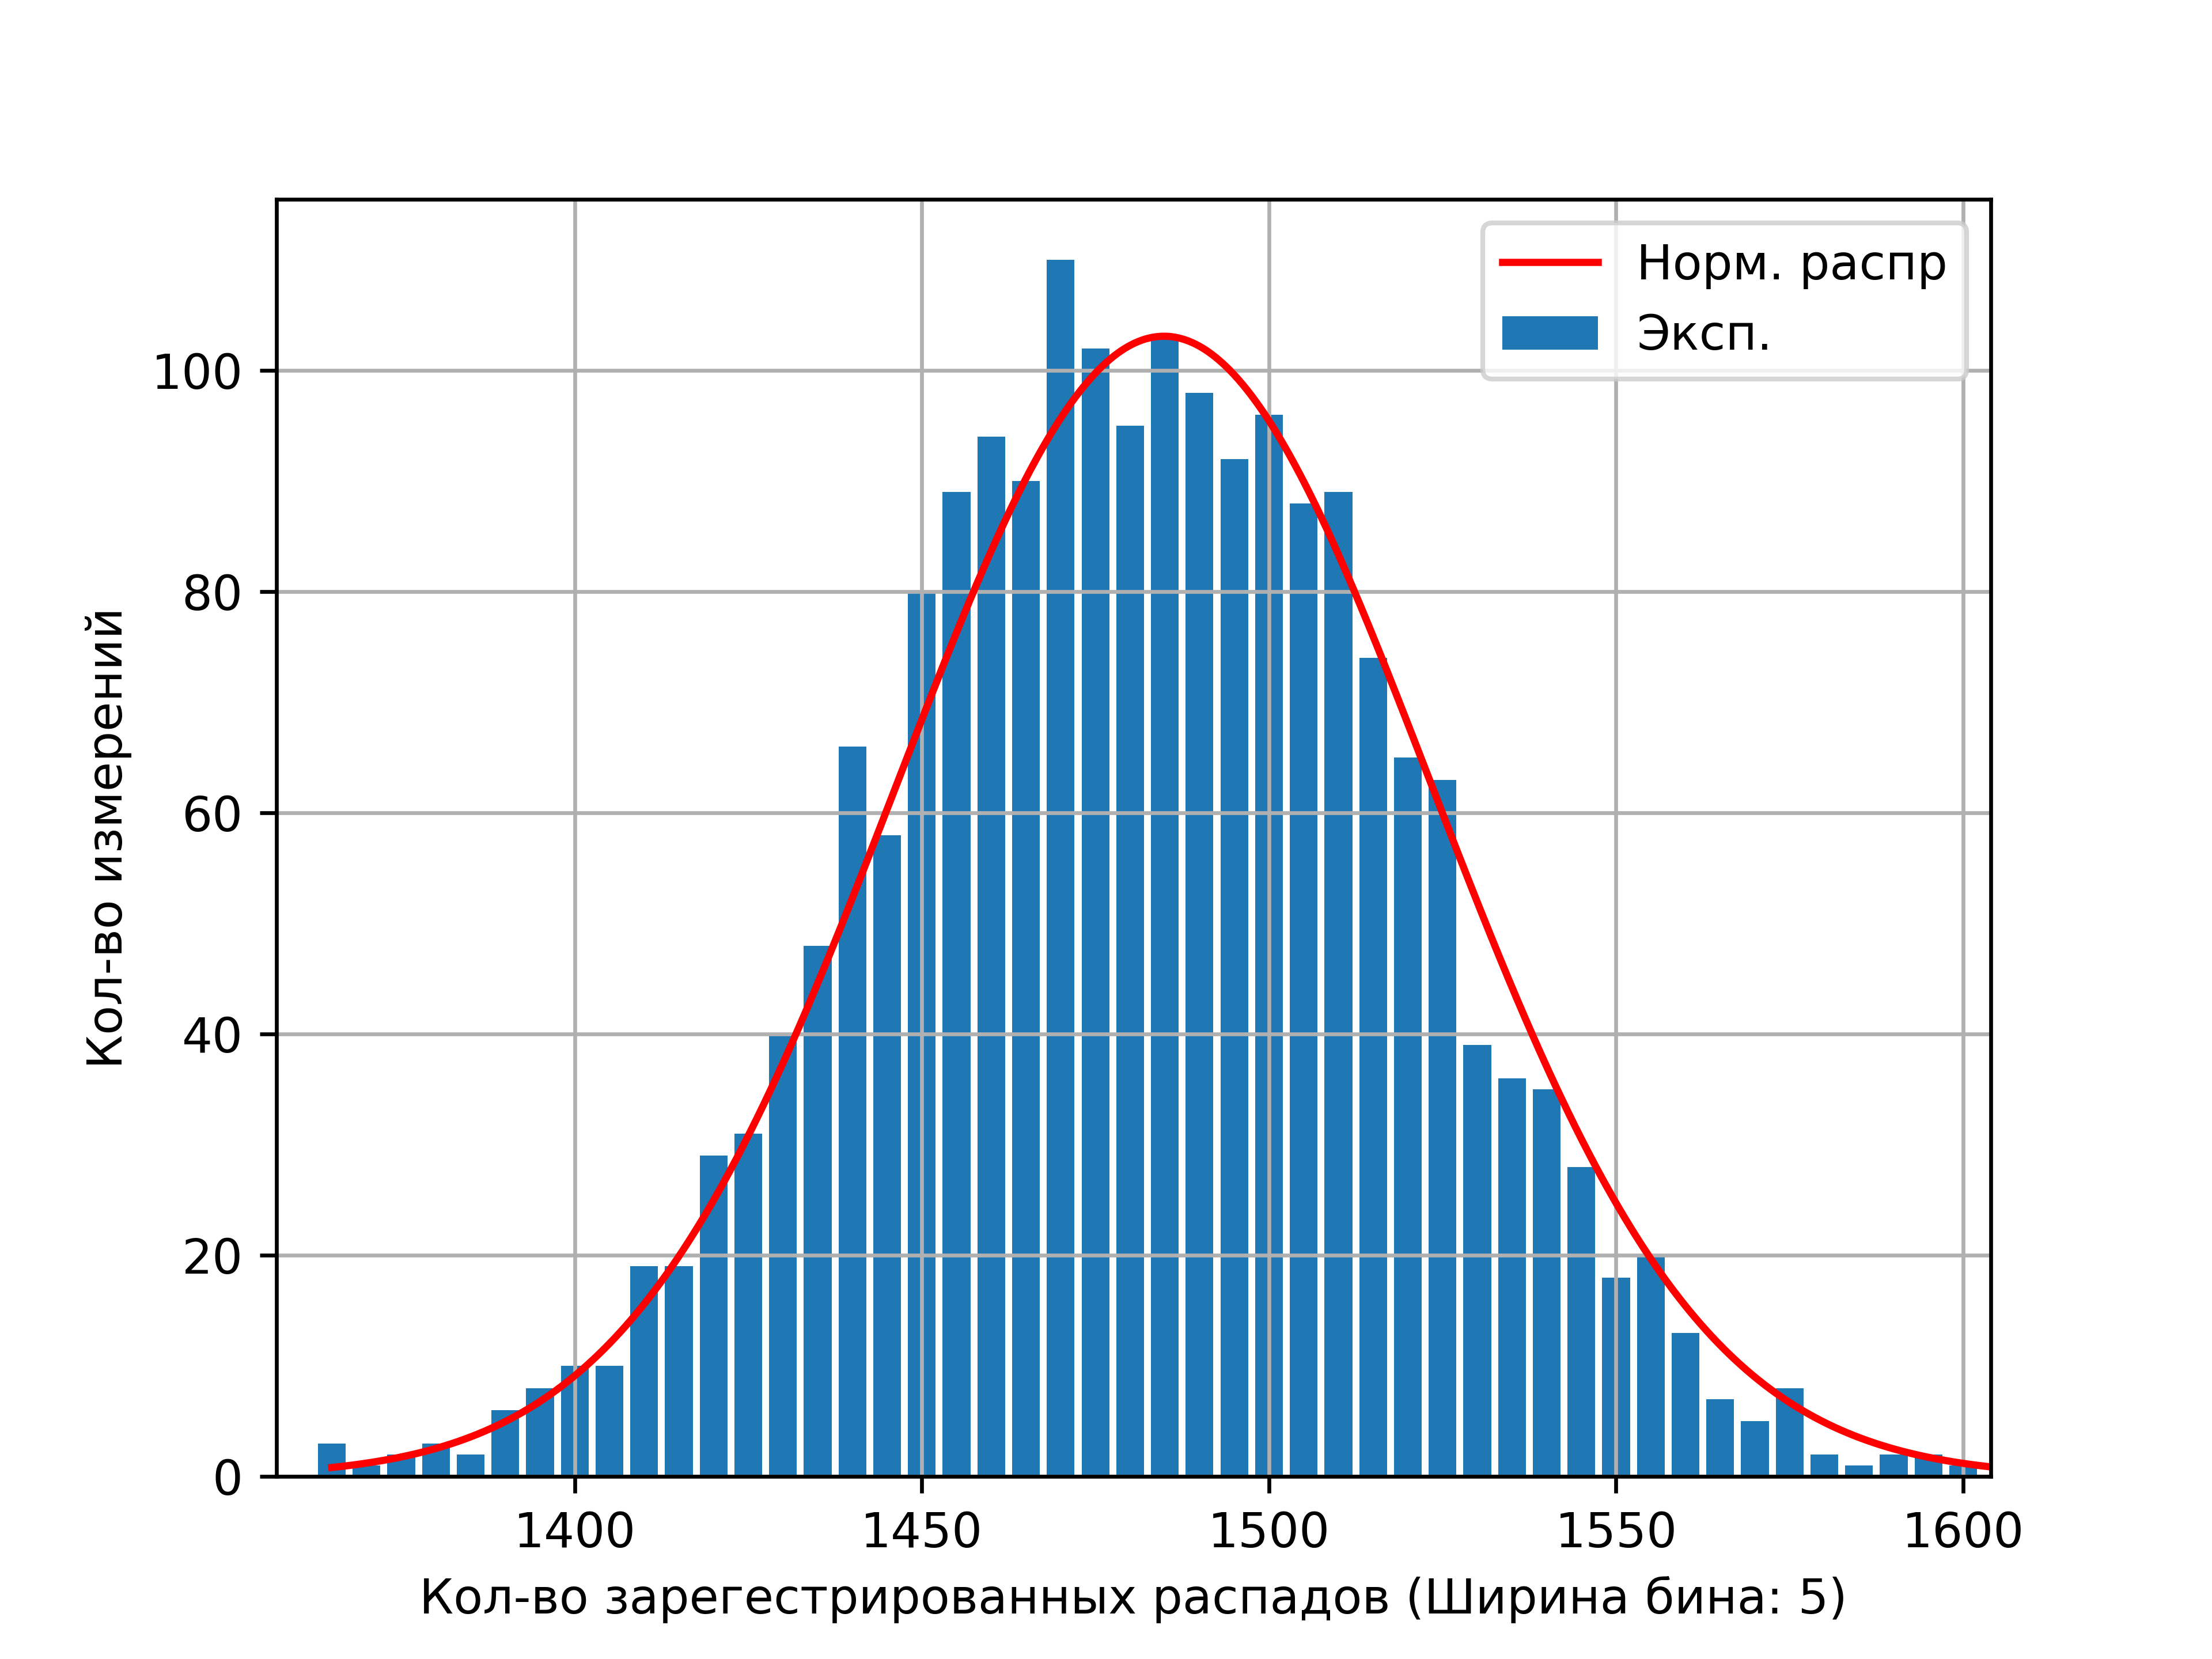
\includegraphics[width=0.5\linewidth]{dt500_n2000.png}
\caption{2000 выборок по 500 мс}
\label{fig:dt500n2000}
\end{figure}
\end{document}